\chapter{Solution design}\label{chapter:soldesign}
This chapter aims to describe the technical details of the developed software, namely the sample page migrate, also referred to SPM throughout this document. The main questions to discuss in this chapter are:
\begin{itemize}
	\item What are the working fundamentals of the SPM tool?
	\item How does the sampling process work?
	\item How is the SPM structured?
\end{itemize}

This chapter develops three parts: Sections \ref{section:ovv-spm} and \ref{section:strat} describe from a very high level point of view the desired functionality and inspiration for the SPM tool, then sections \ref{section:ovv-perfks}, \ref{section:important-structs} and \ref{section:important-structs} describe the sampling acquisition process from a PMU in a Linux environment and finally section \ref{section:spminternals} discussese the design and implementation details of the SPM tool.


\section{Overview of the SPM tool}\label{section:ovv-spm}


\begin{figure}[ht]
	\centering
		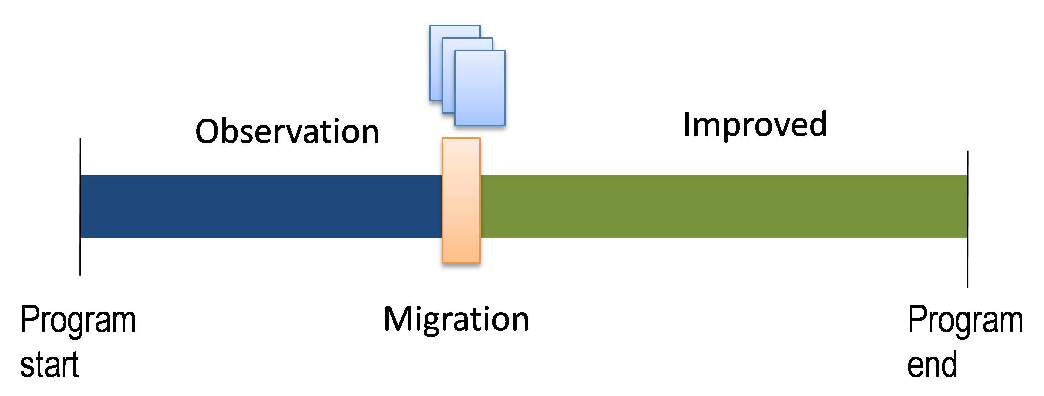
\includegraphics[width=.6\textwidth]{figures/spm-principle.eps}
		\caption[Three phases of execution of the SPM development]{The developed tool consists of three main phases: the observation phase, the page migration phase and the improved phase.}
		\label{fig:sprinciple}
\end{figure}

Figure \ref{fig:sprinciple} shows the high level operation of the SPM tool through time, which has three phases of execution: the \textbf{observation phase}, the \textbf{page migration phase} and the \textbf{improved phase}. During the measuring phase, SPM measures the memory behavior of the guest process, where the length of this process is determined by the user and set in the overall SPM configuration. The page migration will reallocate the home of the pages according to the information obtained in the observation phase and a pre-established policy. The length of the page migration phase depends solely on how long it takes to migrate the pages marked for this process. The improved phase lasts until the end of program execution, where it will again analyze the memory behavior of the program and print information at the end to make possible an assessment over the benefits of the page migration process.

\section{Strategy and alternatives of development}\label{section:strat}
In order to implement the desired functionality the idea is to adapt the code from one of the already working tools that access the PMU to the needs of the project. Two options were considered: \textit{perf} and \textit{numaTop}, with the latter being chosen. It is worth noting that for the communication with the Performance Measurement Unit both tools make use of the same set of library calls. A short description of both alternatives will be given in this chapter.

Figure \ref{fig:dstrategy} shows the overall working principle of the developed tool. The developed tool invokes the configuration capabilities from the kernel side, which then configures the physical PMU. Once configured and started the PMU starts passing samples to the kernel side, which passes them on to the measurement tool once the buffers are read. Upon a read in user space the sample will be passed to the custom tool for processing the samples. The control part will be in charge of coordinating the execution of all the parts of the program.

\begin{figure}[ht]
	\centering
		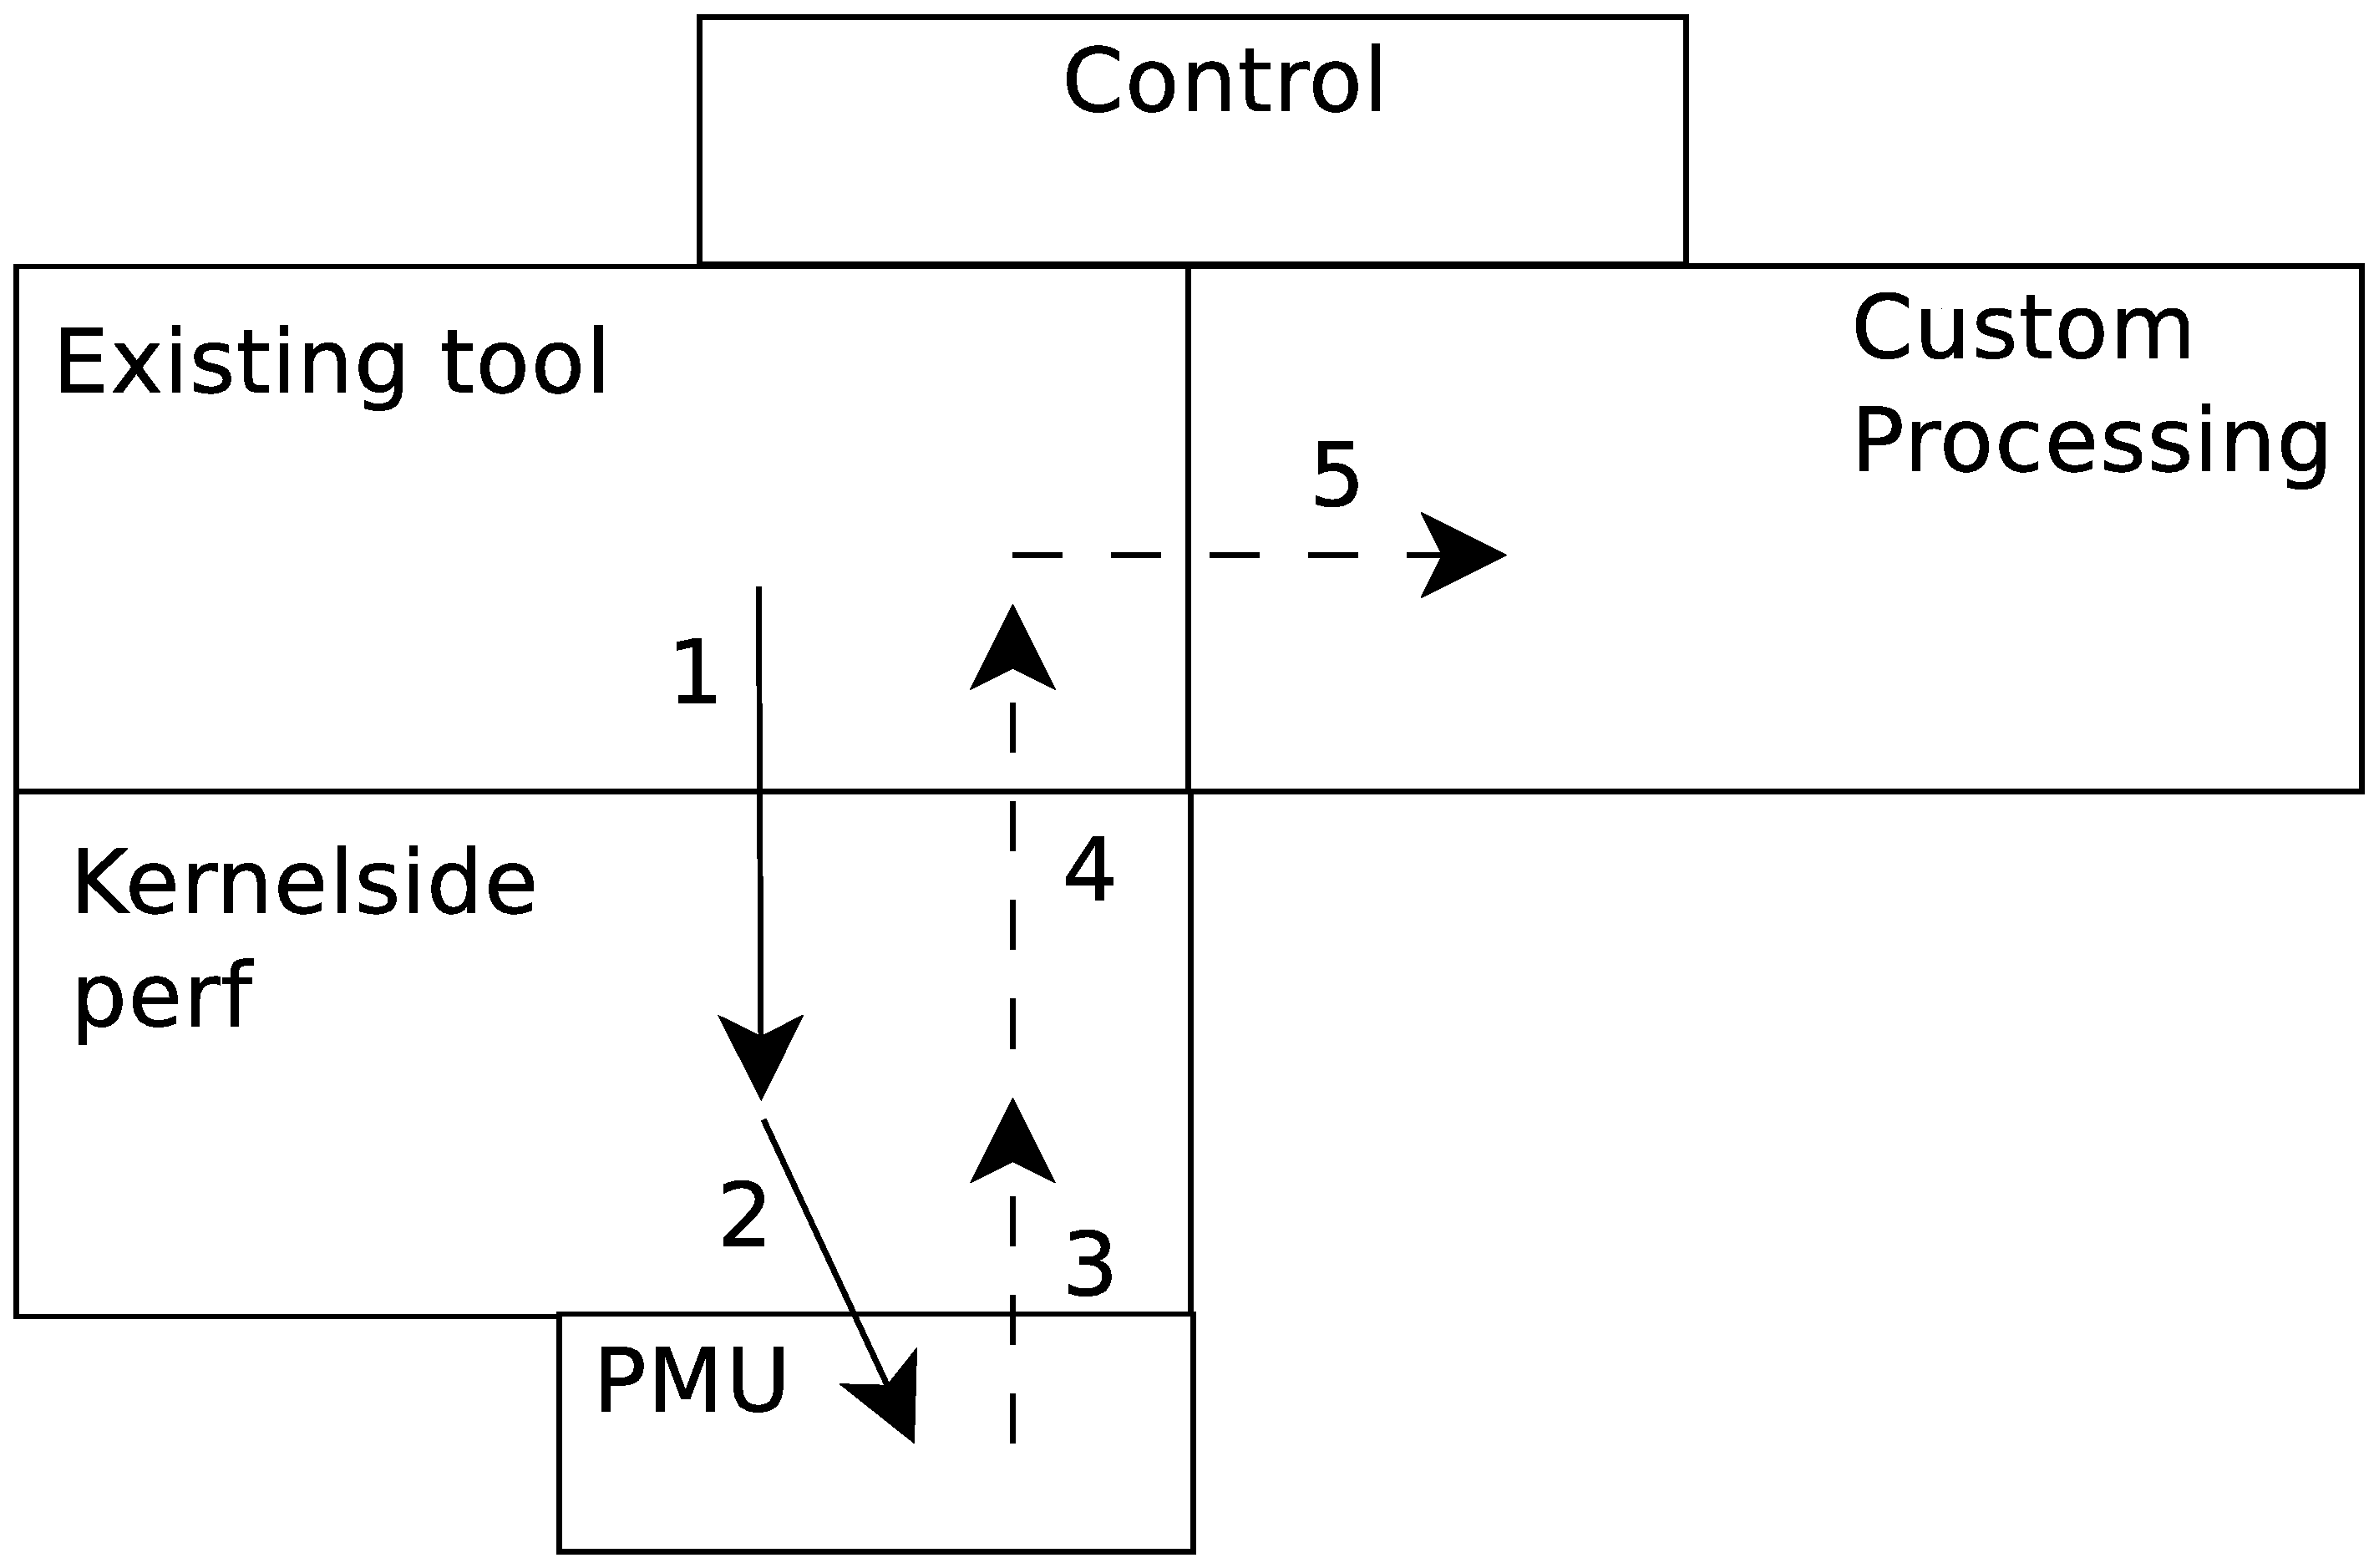
\includegraphics[width=.8\textwidth]{figures/dev-strategy.eps}
		\caption[Flow of information in the development]{Interaction between the parts of the performance measurement. The continuous arrows show the flow of control calls and the dashed line shows the flow of the performance samples.}
		\label{fig:dstrategy}
\end{figure}
\subsection{Perf user tools}\label{section:perf-ut}

This is the most comprehensive covering a diverse range of architectures and performance events. Unfortunately this complexity together with the lack of documentation make the adaptation process a time consuming task and the end solution comprises a great number of source files, which cannot be shrunk without undertaking a large effort. 

The perf user tool \texttt{perf top} was adapted in order to have a constant and never ending access to the samples. In the function \texttt{perf\_event\_process\_samples} in the file builtin\_top.c a call is made to intercept the produced sample and analyzed according to our needs. The GUI of the executable is disabled.

\subsection{NumaTop}\label{section:numatop}
NumaTop provides a reduced functionality in comparison with the user side of perf, but it still provides all the functionality that is needed for this project. Its smaller code size helps to better understand how the sample acquisition process better works. The needed methods were grouped into a smaller file in order to make the number of source files smaller and around this the SPM code was built.

\subsection{Evaluation}\label{section:sol-evltn}
Even though both provide a suitable alternative to the functionality needed, the implementation based on numaTop was chosen mainly because it provides a smaller code base that compiles faster and is easier to understand. 

\section{Communicating with perf's kernel side}\label{section:ovv-perfks}

\begin{figure}
	\centering
		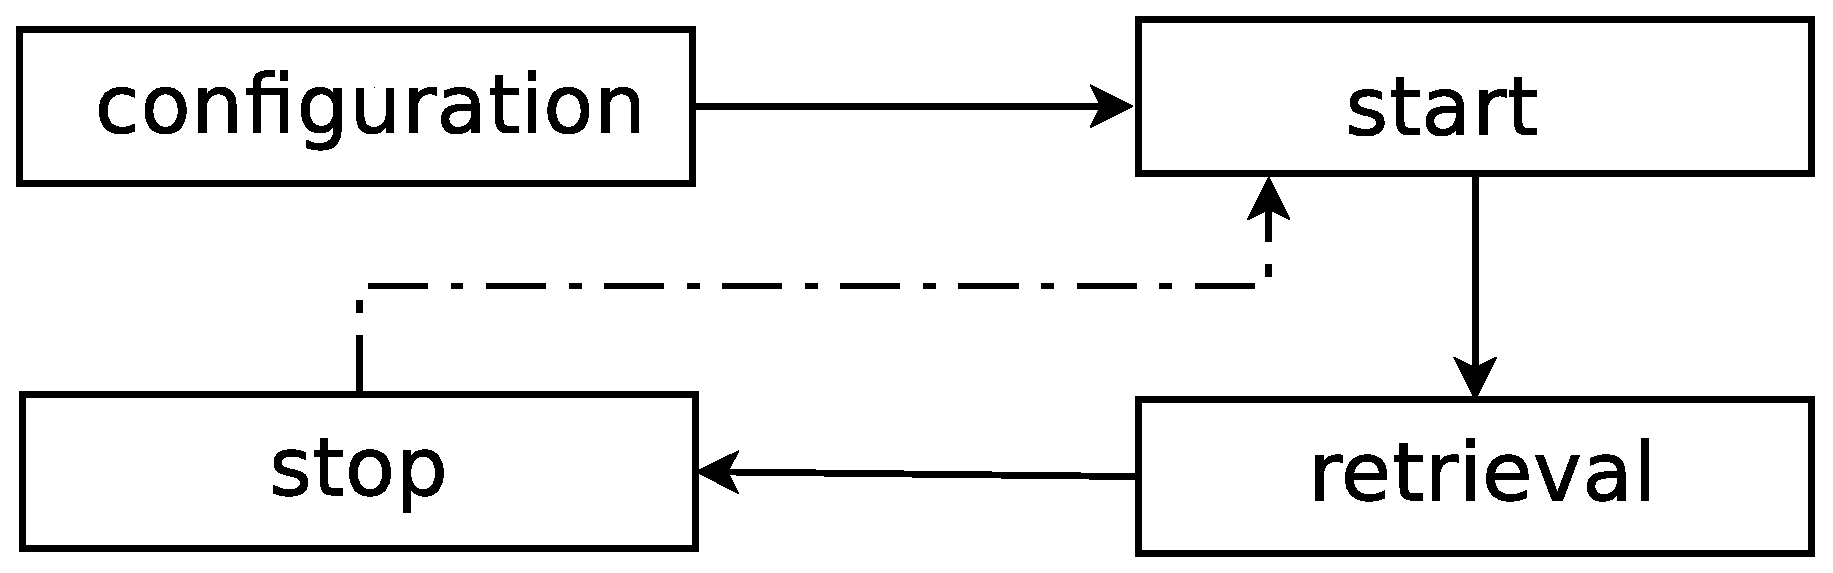
\includegraphics[width=.7\textwidth]{figures/sampling-process.eps}
		\caption[Steps of the performance measurement process]{Steps involved in the performance measurement process, the dashed line means an optional transition.}
		\label{fig:sprocess}
\end{figure}

In order to be able to retrieve samples from the kernel side, a small amount of system calls have to be made. This section describes the flow for using the measuring system and mentions the system calls used. Figure \ref{fig:sprocess} shows an overview of the sampling process with its four stages: configuration, start, retrieval and stop.

\subsection{Configuration}\label{section:confgtn}
The configuration of the PMU is made for every event and for every CPU that is to be watched, by making the system call with identifier \_\_NR\_perf\_event\_open. An actual call would take the form: 
\\
\begin{center}
\texttt{syscall(\_\_NR\_perf\_event\_open, attr, pid, cpu, group\_fd, flags) }
\end{center}

\begin{itemize}
	\item Attr: A struct of type \texttt{perf\_event\_attr} which specifies the sampling parameters, its fields are better explained in section \ref{section:important-structs}. 
	\item Pid: Takes the value -1, in order to be able to monitor all the executing PIDs.
	\item CPU: Takes the identifier of the core whose PMU is to be configured.
	\item Group\_fd: For this implementation takes the value -1.
	\item Flags: For this implementation it takes the value 0.
\end{itemize}

After setting up the PMU the function \textbf{mmap} is called in order to create a file descriptor, which will be used to read the samples. In order to create the descriptor, the first parameter of the mmap function call is NULL. The most important parameter in the PMU set up is the attr field, because it specifies what we want to measure. The most important fields of this struct are explained in section \ref{section:pea-stru}.  

\subsection{Start and stop of the sampling}\label{section:start-sto}

To start and stop the sample unit the following system call is made: 
\\
\begin{center}
\texttt{ioctl(descriptor, constant, 0)}
\end{center}
Where descriptor is the file descriptor assigned to every combination of CPU and event and constant takes the value PERF\_EVENT\_IOC\_DISABLE or PERF\_EVENT\_IOC \_ENABLE depending on the desired action.


\subsection{Retrieval and the reading the samples}\label{section:retr-reaf}

The file descriptor must be read periodically in order to collect samples. Given that the acquisition of the samples is made through low level I/O, the read is made by reading a chunk of certain number of bytes and it is up to the programmer to turn this stream into a suitable representation. 

The read of the descriptor is made using the \textbf{mmap} function, which takes as parameter the descriptor, the length of the read and the buffer where the read information will be kept.

\subsection{The numatop core}\label{section:numatop-core}
The SPM tool is based on an adaptation of the numatop functions used for communicating with the perf kernel side. This functions are located in the \textit{sampling-core.c} file of the SPM sources, or on the numatop sources themselves.

The functions follow the logic described in section \ref{section:ovv-perfks} and they exist in two varieties: the methods with \textbf{profiling} in their name refer to the access of the registers that refer to a sampling value, such as the access to the offcore registers and the methods with \textbf{ll} refer to the load latency records, which are precise methods. Their functionality is very similar. 

\section{Important data structures}\label{section:important-structs}

\subsection{The perf\_event\_attr struct}\label{section:pea-stru}

The \textbf{perf\_event\_attr} is the struct used to configure the PMU as shown in section \ref{section:ovv-perfks}. In its fields the configuration parameters of the PMU are set. As it has a relatively high number of fields, only the most important will be explained here. For the complete description of this struct it is advisable to check the man pages of the \textit{sys\_perf\_event\_open} call and the document \textit{design.txt} located on the root of the perf user side source tree. This struct is defined in the kernel header \textit{perf\_event.h}. 
\begin{itemize}
	\item record\_type: For the use in our program will always take the value 4 (PERF\_TYPE \_RAW) since we are retrieving data only from the hardware PMU. It is possible to collect data from other sources, such as the kernel itself, for instance.
	\item sample\_period: Specifies the number of instructions between consecutive samples. It is also possible to specify a frequency instead of a period by setting the \textit{use\_freq} field.
	\item Precise\_ip: It is used to specify that the event to be read uses precise sampling(see section \ref{subsection:sampling}).
	\item Config and config1: Config specifies the event to read as it is formed by concatenating the umask and the id. Config1 is used to specify any additional information that a specific event requires. 
	\item Sample\_type: This field consists of the logic OR of the chosen fields specified in the \textit{perf\_event\_sample\_format} enumeration and determines which information is returned in every sample, for example PERF\_SAMPLE\_IP | PERF\_SAMPLE\_TID | and so forth.
	\item Disabled: Determines whether the sampling requires further additional activation or starts immediately after the configuration call.
\end{itemize}
     
\subsection{A perf sample}\label{section:pf-samplu}
     
The samples are retrieved from a sequential read to a file descriptor, so it is up to the programmer to give sense to this incoming information. The first information coming from a sample is the header, which follows the layout of the struct \textit{perf\_event\_header}. From this header we obtain two important pieces of information: the first one is the size of the sample and the other is the type of the sample. For the type of the sample and our purposes it is only important the samples of type PERF\_RECORD\_SAMPLE. Once read the header, the next size bytes will belong to the payload of a sample.

The information coming in a sample is determined by what was configured in the \textit{sample\_type} field when configuring the sampling. What is still unknown is the order in which the fields are returned. In order to figure this out it is better to refer to an existing implementation. For the consumption of the sample body, the idea is to read each field and displace the reading position the number of bytes that a field occupies. The functions \textit{profiling\_sample\_read} and \textit{ll\_sample\_read} provide the sample reads that are used in the development. 


\begin{itemize}
	\item The functions responsible for setting up the PMU are \textit{pf\_profiling\_setup} and \textit{cpu\_ll \_setup}.
	\item The functions responsible for starting the PMU are \textit{pf\_profiling\_start} and \textit{pf\_ll \_start}. 
	\item The functions responsible for stopping the PMU are \textit{pf\_profiling\_stop} and \textit{pf\_ll \_stop}.
\end{itemize}
  
\section{Internals of the spm tool}\label{section:spminternals}

\subsection{Layout of the spm tool }\label{subsection:main-layout}
\begin{figure}[h]
	\centering
		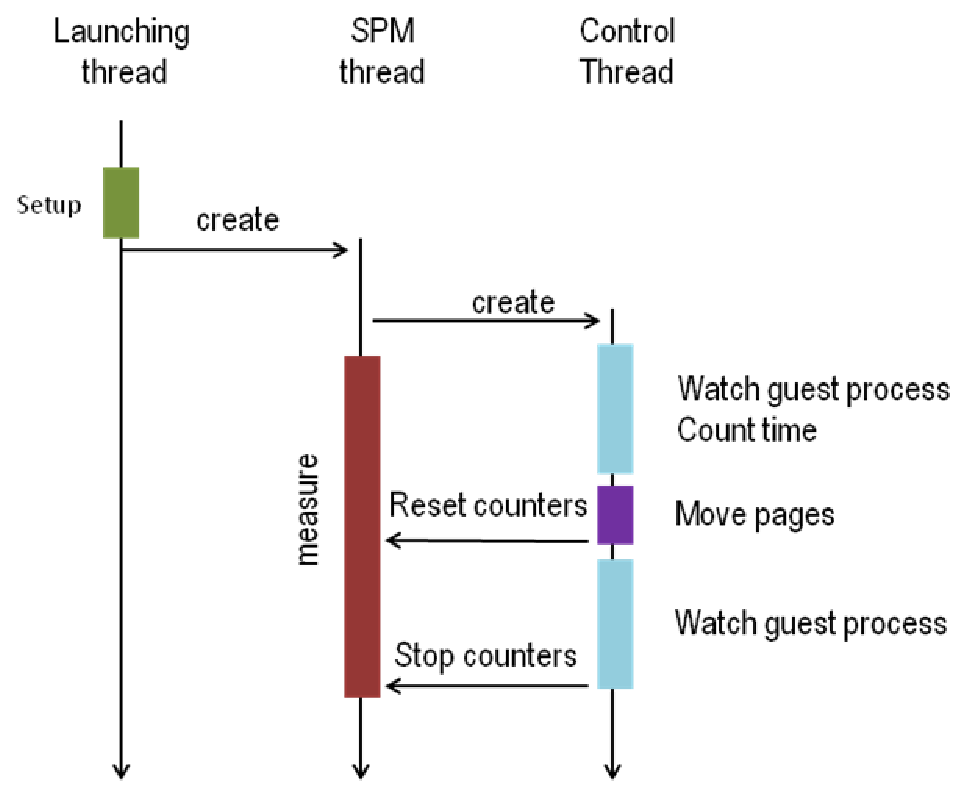
\includegraphics[width=.9\textwidth]{figures/sequence.eps}
		\caption[Timing and threads in the execution of the SPM tool]{Interaction between SPM's three threads showing the functionality through time}
		\label{fig:sol-seq}
\end{figure}

Figure \ref{fig:sol-seq} shows the overall principle of implementation of the SPM tool: The \textbf{launching thread} sets up the system and creates the \textbf{SPM thread}, which is in charge of collecting the samples from the numaTop core. The SPM thread then will launch the \textbf{control thread}, which controls the overall execution of the three phases, prints the statistics, invokes the migration and ensures that the observed process is executing on the background.

\subsection{Structure of the spm tool}\label{subsection:spmstructr}

The SPM tool consists of the following files:
\begin{itemize}
	\item spm.h: Contains struct declarations and function prototypes.
	\item sampling-core.c: Contains the core functions from numatop that access the PMU.
		\item perf\_helpers.c: Contains a few functions borrowed from perf's user side tools.
	\item sample-processing.c: Contains the functions related to the processing of a sample.
	\item perf\_helpers.c: Contains a few functions borrowed from perf's user side tools.
	\item sample-processing.c: Contains the functions related to the processing of a sample.
	\item control.c: Contains the logic that controls the whole execution lifetime of the SPM tool.
\end{itemize}

\subsection{Information collected by the SPM tool}\label{subsection:spminf}

The information shown by SPM at the end of a measurement round is as follows:
Total number of samples taken in the phase and number of samples collected belonging to the observed process.
\begin{itemize}
	\item Number of remote candidate and total samples taken for every core.
	\item Breakdown of samples taken by access type: How many samples are L1 hits, L2 hits, remote access and so forth.
	\item Histogram of frequency of page accesses, that is a detail of how many pages were accessed a given time
	\item Histogram of the number of pages with a latency value that belong to a certain interval. During this document the access weights are placed on intervals of 50.
\end{itemize}

\subsection{Overview of the sample processing performed by SPM}\label{subsection:ov-samplproc}
The samples are retrieved from the numatop functionality in the read\_samples function. From there the consume\_sample function is invoked, which collects all the needed information from a sample: 

\begin{itemize}
	\item The counter for the total number of samples is increased, as well as the number of samples per core.
	\item Only the samples that belong to the PID we are interested in are further processed.
	\item From the data\_source field of a sample the type of access is derived. L1, L2 and L3 hits are not further processed because they are local accesses. This type of access is added to the type of access histogram.
	\item From the latency value an entry is added to its corresponding interval in the latency histogram.
	\item If the address of the page contained in the sample belongs to a candidate remote access, that page address will be added to the hash table of page accesses, which are used as candidates for a page migration. If the entry already exists it will be retrieved and an access belonging to the originating core will be registered, otherwise it will be created and incorporated into the hash table.
\end{itemize}



\subsection{Access to the SPM functionality}\label{subsection:spm-access}
The SPM functionality is engaged by simply calling the function: 

\begin{center}
\texttt{int init\_spm(struct sampling\_settings *ss)} 
\end{center}

where it takes as a parameter a properly filled struct of type sampling\_settings.

\subsection{Configuration of the SPM settings}\label{subsection:spm-settings}
The configuration of SPM is passed as start time to the \textit{init\_spm} function as a pointer to a struct of type \textit{sampling\_settings}, whose fields have the following meaning:

\begin{itemize}
\item int pid\_uo: Indicates the process id of the observed process. If its value is equal or less than 0, SPM will launch the command indicated in command2launch and fill this field automatically.
\item int *core\_to\_cpu: This field contains an array whose value at position n represents the NUMA node to which core n belongs, it is filled automatically at configuration time.
\item const char** command2\_launch: Specifies a command to launch by SPM together with its arguments. If a pid is specified it is not necessary to specify it.
\item char* output\_label: Used to prepend a label to the statistics print by the tool, useful when using automatic processing of the results.
\item Int argv\_size: Size of the command2\_launch array.
\item int measure\_time: Time in seconds that the measure phase will last.
\item boolean\_t only\_sample: Used to indicate SPM to run only a observation phase, without page migration.
\item int ll\_sampling\_period: Contains the sampling period of the precise registers.
\item int ll\_weight\_threshold: Samples below this value are ignored, must be greater than 3.
\end{itemize}
The following fields are meant only for internal use of the tool:
\begin{itemize}
	\item int n\_cpus: This field contains the number of NUMA nodes in the system.
\item int n\_cores: This field contains the number of cores in the system.
\item perf\_cpu\_t *cpus\_ll: File descriptor to access the load latency registers.
\item perf\_cpu\_t *cpus\_pf: File descriptor to access the non-precise registers.
\item boolean\_t end\_recording: Internal flag to signal the sampling system that sampling should be ended.
\item struct l3\_addr *pages\_2move: Contains a linked list with all the pages candidates to be moved.
\item int number\_pages2move: Contains the size of the pages\_2move list.
\item int moved\_pages: Contains how many pages were moved.
\item struct sampling\_metrics: Contains many structures used for handling the statistics.
\end{itemize}
\subsection{Page migration procedure} \label{subsection:pm-proc}

Once the control invokes the do\_great\_migration function, the following procedure will be followed:

\begin{enumerate}
	\item The hash table with the possible remote accesses is used to fill an array with all the candidate addresses. This must be done because the candidates of type L3 miss might be accesses to local memory or accesses to the memory of a remote node, so it is necessary to retrieve further information on the nature of the access. This is accomplished by calling the move\_pages function in query mode, where it returns an array with the NUMA node where the page is currently located.
	\item With the owner node and page access information, the function will decide whether the page should be moved or not. In the affirmative case its address will be placed in an array, and a subsequent call in move mode will be made.
	\item The new location of the pages that were moved will be checked in order to make sure that the page was moved.
\end{enumerate}

\subsection{Integration with Autopin+}\label{subsection:apinplu-intgr}

The SPM functionality is integrated into the code base of autopin+. For this purpose SPM’s sources are added to the ccmake configuration script \textit{CMakeLists.txt}. For the calling of the SPM functionality within autopin+, a few additions to its code are done:

\begin{enumerate}
	\item A new descendant of the \textit{PerformanceMonitor} class is created, which is then named PageMigrate.
	\item The recognition of the new class is enabled by adding the corresponding logic in the selection \texttt{if} present in the \textit{createPerformanceMonitors} method located in the \textit{Watchdog} class.
	\item A new field is added to the \textit{PerformanceMonitor} class together with the setter method, which allows it to retain the identifier of the process to watch. This is necessary because until now a performance monitor is enabled using the identifier of a thread and in the SPM tool the pid is employed to enable the tool.
	\item The start method is modified in order to invoke the \textit{init\_spm} function. Before the invocation the configuration struct is created and the necessary fields are filled.
\end{enumerate}
